\documentclass{beamer}

\usetheme{Antibes}
\setbeamertemplate{headline}{}
\setbeamertemplate{navigation symbols}{}

\setbeamertemplate{footline}{
	\leavevmode%
	\hbox{%
		\begin{beamercolorbox}[wd=.5\paperwidth,ht=2.5ex,dp=1ex]{title in head/foot}
			\hspace{0.7em}
			\insertframenumber/\inserttotalframenumber
			\hfill
			Νικόλας Μαυρογενειάδης
			\hspace{0.7em}
		\end{beamercolorbox}%
		\begin{beamercolorbox}[wd=.5\paperwidth,ht=2.5ex,dp=1ex]{author in head/foot}
			\hspace{0.7em}
			Κλασικά προβλήματα ταιριάσματος και ταιριάσματα \en Pareto\gr
			\hfill
		\end{beamercolorbox}%
	}%
}

\usepackage{amsthm, amssymb, amsfonts, amsmath}
\usepackage{graphicx}
\usepackage{tikz}
\usetikzlibrary{calc,shapes}
%\usepackage{enumitem}
\usepackage{mathtools}
\usepackage{mathrsfs}
\usepackage{tikz-cd}
\usepackage{xcolor}
\usepackage{listings}
\usepackage{fontspec}
\setmainfont{CMU Serif}
\setsansfont{CMU Sans Serif}
\usepackage[english,greek]{babel}
\usepackage{subfig}
\usepackage{algorithm}
%\usepackage{indentfirst}
\usepackage{fancyhdr}
\usepackage{makeidx}
\makeindex
\usepackage{float}
\usepackage[nameinlink]{cleveref}
\usepackage{url}
\usetikzlibrary{positioning,arrows.meta}
\setlength{\parindent}{2em}

\newcommand{\en}{\selectlanguage{english}}
\newcommand{\gr}{\selectlanguage{greek}}
%Information to be included in the title page:
\gr
\title[Nikolas-Mavrogeneiadis - Thesis]{ %optional
	Ταιριάσματα με και χωρίς προτιμήσεις,\\
	ταιριάσματα Pareto:\\
	Προβλήματα, δομική και πολυεδρική ανάλυση\\
	και αλγόριθμοι επίλυσης
}

\subtitle{Διπλωματική Εργασία}

\author[Ν. Μαυρογενειάδης]
{Νικόλας Μαυρογενειάδης}

\institute[ΠΑΔΑ] 
{
	Τμήμα Μηχανικών Πληροφορικής και Υπολογιστών\\
	Πανεπιστήμιο Δυτικής Αττικής
}

\date[14 Ιουλίου 2026]
{14 Ιουλίου 2026}

\logo{
\includegraphics[height=1cm]{logo}}

\begin{document}
	\gr
	\frame{\titlepage}
	
	\begin{frame}
		\frametitle{Αντικείμενο της διπλωματικής}
		
		Η διπλωματική μελετά προβλήματα ταιριάσματος σε γράφους.
		
		\vspace{0.3cm}
		
		Στόχος είναι να δούμε πώς τέτοια προβλήματα μπορούν να αντιμετωπιστούν:
		\begin{itemize}
			\item αλγοριθμικά,
			\item μέσω γραμμικού και ακέραιου προγραμματισμού,
			\item και, στο τελευταίο μέρος, μέσω πολυεδρικής και υπολογιστικής ανάλυσης.
		\end{itemize}
	\end{frame}
	
	\begin{frame}
		\frametitle{Ταιριάσματα}
		
		Τα ταιριάσματα αποτελούν έναν φυσικό τρόπο μοντελοποίησης προβλημάτων ανάθεσης.
		
		\vspace{0.3cm}
		
		Για παράδειγμα, μπορεί να θέλουμε να αντιστοιχίσουμε:
		\begin{itemize}
			\item δασκάλους σε σχολεία,
			\item υποψηφίους σε κατοικίες,
			\item φοιτητές, καθηγητές και projects.
		\end{itemize}
		
		\vspace{0.3cm}
		
		Οι απαιτήσεις κάθε προβλήματος μπορεί να διαφέρουν σημαντικά ανάλογα με την εφαρμογή.
	\end{frame}
	
	\begin{frame}
		\frametitle{Δύο βασικές προσεγγίσεις}
		
		Η εργασία ακολουθεί δύο βασικές οπτικές.
		
		\vspace{0.3cm}
		
		\begin{itemize}
			\item \textbf{Αλγοριθμική προσέγγιση:}  
			μελετάμε αλγορίθμους που κατασκευάζουν τα ζητούμενα ταιριάσματα.
			
			\vspace{0.2cm}
			
			\item \textbf{Προσέγγιση μέσω γραμμικού προγραμματισμού:}  
			διατυπώνουμε τα προβλήματα ως ακέραια προγράμματα και μελετάμε τις γραμμικές χαλαρώσεις τους.
		\end{itemize}
	\end{frame}
	
	\begin{frame}
		\frametitle{Πρώτο μέρος της εργασίας}
		
		Στο πρώτο μέρος μελετάμε δύο κλασικά προβλήματα ταιριάσματος.
		
		\vspace{0.3cm}
		
		\begin{itemize}
			\item Το πρόβλημα του μέγιστου ταιριάσματος σε διμερείς γράφους.
			\item Το πρόβλημα του σταθερού γάμου.
		\end{itemize}
		
		\vspace{0.3cm}
		
		Για αυτά τα προβλήματα παρουσιάζουμε τόσο την αλγοριθμική πλευρά όσο και τη διατύπωσή τους μέσω γραμμικού και ακέραιου προγραμματισμού.
	\end{frame}
	
	\begin{frame}
		\frametitle{Δεύτερο μέρος της εργασίας}
		
		Στο δεύτερο μέρος μελετάμε Pareto βέλτιστα ταιριάσματα σε ένα μοντέλο ανάθεσης κατοικιών.
		
		\vspace{0.3cm}
		
		Σε αυτό το μοντέλο:
		\begin{itemize}
			\item μόνο οι applicants έχουν προτιμήσεις,
			\item οι κατοικίες είναι αδιαίρετα αντικείμενα,
			\item και μας ενδιαφέρει η έννοια της Pareto βελτιστότητας.
		\end{itemize}
	\end{frame}
	
	\begin{frame}
		\frametitle{Στόχος του δεύτερου μέρους}
		
		Στο μοντέλο των Pareto βέλτιστων ταιριασμάτων, η γραμμική χαλάρωση είναι πιο σύνθετη.
		
		\vspace{0.3cm}
		
		Η εργασία μελετά:
		\begin{itemize}
			\item τη γραμμική χαλάρωση του αντίστοιχου ακέραιου προγράμματος,
			\item το πρόβλημα διαχωρισμού για μια μεγάλη οικογένεια περιορισμών,
			\item και την πραγματική κυρτή θήκη των Pareto βέλτιστων ταιριασμάτων για μικρά instances.
		\end{itemize}
	\end{frame}
	
	\begin{frame}
		\frametitle{Μέγιστο ταίριασμα σε διμερείς γράφους}
		
		Έστω ένας διμερής γράφος
		\[
		G=(V_1\cup V_2,E).
		\]
		
		Ένα \textbf{ταίριασμα} είναι ένα σύνολο ακμών, στο οποίο κάθε κορυφή συμμετέχει σε το πολύ μία ακμή.
		
		\vspace{0.3cm}
		
		Στόχος του προβλήματος είναι να βρούμε ένα ταίριασμα μέγιστης πληθικότητας, δηλαδή ένα ταίριασμα που περιέχει τον μεγαλύτερο δυνατό αριθμό ακμών.
	\end{frame}
	
	\begin{frame}
		\frametitle{Μέγιστο και μεγιστικό ταίριασμα}
		
		Ένα ταίριασμα $M$ ονομάζεται:
		
		\begin{itemize}
			\item \textbf{μεγιστικό}, αν δεν μπορεί να προστεθεί κάποια ακμή χωρίς να παραβιαστεί η ιδιότητα του ταιριάσματος,
			
			\item \textbf{μέγιστο}, αν κανένα άλλο ταίριασμα δεν έχει περισσότερες ακμές.
		\end{itemize}
		
		\vspace{0.3cm}
		
		Κάθε μέγιστο ταίριασμα είναι μεγιστικό, αλλά το αντίστροφο δεν ισχύει πάντα.
	\end{frame}
	
	\begin{frame}
		\frametitle{Εναλλασσόμενα και αυξητικά μονοπάτια}
		
		Ένα μονοπάτι ονομάζεται \textbf{εναλλασσόμενο} ως προς ένα ταίριασμα $M$, όταν οι ακμές του ανήκουν εναλλάξ στο $M$ και στο $E\setminus M$.
		
		\vspace{0.3cm}
		
		Ένα εναλλασσόμενο μονοπάτι ονομάζεται \textbf{αυξητικό} όταν:
		
		\begin{itemize}
			\item τα δύο άκρα του είναι ελεύθερες κορυφές,
			\item η πρώτη και η τελευταία ακμή του δεν ανήκουν στο $M$.
		\end{itemize}
		
		\vspace{0.3cm}
		
		Αν εναλλάξουμε τις ακμές ενός αυξητικού μονοπατιού, η πληθικότητα του ταιριάσματος αυξάνεται κατά μία.
	\end{frame}
	
	\begin{frame}
		\frametitle{Θεώρημα του Berge}
		
		Το βασικό αποτέλεσμα πάνω στο οποίο στηρίζονται οι αλγόριθμοι είναι το θεώρημα του Berge.
		
		\begin{block}{Θεώρημα του Berge}
			Ένα ταίριασμα $M$ είναι μέγιστο αν και μόνο αν δεν υπάρχει αυξητικό μονοπάτι ως προς το $M$.
		\end{block}
		
		\vspace{0.3cm}
		
		Επομένως, το πρόβλημα της εύρεσης μέγιστου ταιριάσματος μπορεί να αντιμετωπιστεί αναζητώντας επανειλημμένα αυξητικά μονοπάτια.
	\end{frame}
	
	\begin{frame}
		\frametitle{Αλγόριθμος αυξητικών μονοπατιών}
		
		Ο βασικός αλγόριθμος ξεκινά από το κενό ταίριασμα και επαναλαμβάνει τα εξής βήματα:
		
		\begin{enumerate}
			\item Επιλέγει μία ελεύθερη κορυφή του $V_1$.
			\item Αναζητά με DFS ένα αυξητικό μονοπάτι προς μία ελεύθερη κορυφή του $V_2$.
			\item Αν βρεθεί τέτοιο μονοπάτι, εναλλάσσει τις ακμές του.
		\end{enumerate}
		
		\vspace{0.3cm}
		
		Όταν δεν υπάρχει πλέον αυξητικό μονοπάτι, το θεώρημα του Berge εγγυάται ότι το ταίριασμα είναι μέγιστο.
	\end{frame}
	
	\begin{frame}
		\frametitle{Πολυπλοκότητα του βασικού αλγορίθμου}
		
		Μία αναζήτηση αυξητικού μονοπατιού εξετάζει κάθε κορυφή και κάθε ακμή το πολύ μία φορά.
		
		\vspace{0.3cm}
		
		Η αναζήτηση εκτελείται για κάθε κορυφή του $V_1$. Επομένως, η συνολική πολυπλοκότητα είναι
		\[
		O(nm),
		\]
		όπου $n$ είναι ο αριθμός των κορυφών και $m$ ο αριθμός των ακμών.
		
		\vspace{0.3cm}
		
		Ο αλγόριθμος είναι απλός, αλλά αυξάνει το ταίριασμα κατά μία μόνο ακμή σε κάθε επιτυχημένη αναζήτηση.
	\end{frame}
	
	\begin{frame}
		\frametitle{Αλγόριθμος Hopcroft--Karp}
		
		Ο Hopcroft--Karp βελτιώνει τον βασικό αλγόριθμο, βρίσκοντας πολλά αυξητικά μονοπάτια σε κάθε φάση.
		
		\vspace{0.3cm}
		
		Κάθε φάση αποτελείται από δύο βασικά βήματα:
		
		\begin{enumerate}
			\item Με BFS κατασκευάζεται ένα πολυεπίπεδο δίκτυο που περιγράφει τα συντομότερα αυξητικά μονοπάτια.
			\item Με DFS εντοπίζεται ένα μεγιστικό σύνολο κορυφοξένων συντομότερων αυξητικών μονοπατιών.
		\end{enumerate}
		
		\vspace{0.3cm}
		
		Οι ακμές όλων αυτών των μονοπατιών εναλλάσσονται ταυτόχρονα.
	\end{frame}
	
	\begin{frame}
		\begin{figure}[h]
				\centering
				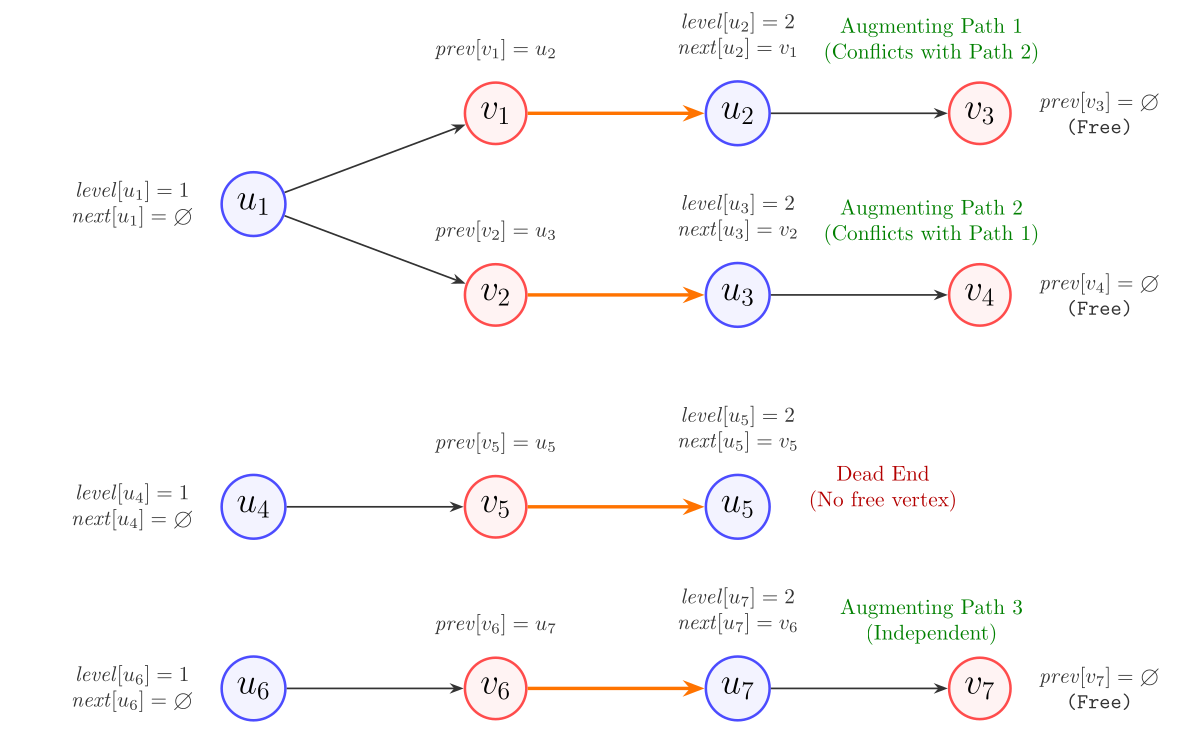
\includegraphics[width=1.0\textwidth]{pic1}
				\caption{Πολυεπίπεδο Δίκτυο}
				\label{fig:mesh1}
		\end{figure}
	\end{frame}
	
	
	
	
	\begin{frame}
		\frametitle{Πολυπλοκότητα του Hopcroft--Karp}
		
		Κάθε φάση του Hopcroft--Karp απαιτεί
		\[
		O(n+m)
		\]
		χρόνο.
		
		\vspace{0.3cm}
		
		Επιπλέον, ο αριθμός των φάσεων είναι
		\[
		O(\sqrt{n}).
		\]
		
		\vspace{0.3cm}
		
		Άρα η συνολική πολυπλοκότητα είναι
		\[
		O\bigl((n+m)\sqrt{n}\bigr).
		\]
		
		Ο Hopcroft--Karp είναι σημαντικά ταχύτερος από τον βασικό αλγόριθμο αυξητικών μονοπατιών για μεγάλους διμερείς γράφους.
	\end{frame}
	
	\begin{frame}
		\frametitle{Σύνδεση με το πρόβλημα μέγιστης ροής}
		
		Το πρόβλημα μέγιστου διμερούς ταιριάσματος μπορεί επίσης να αναχθεί σε πρόβλημα μέγιστης ροής.
		
		\vspace{0.3cm}
		
		Κατασκευάζουμε ένα δίκτυο προσθέτοντας:
		
		\begin{itemize}
			\item μία πηγή που συνδέεται με όλες τις κορυφές του $V_1$,
			\item μία καταβόθρα στην οποία συνδέονται όλες οι κορυφές του $V_2$,
			\item χωρητικότητα ίση με $1$ σε κάθε ακμή.
		\end{itemize}
		
		\vspace{0.3cm}
		
		Η τιμή μιας μέγιστης ακέραιας ροής στο δίκτυο είναι ίση με την πληθικότητα ενός μέγιστου ταιριάσματος στον αρχικό γράφο.
	\end{frame}
	
	\begin{frame}
		\frametitle{Βασικά αποτελέσματα}
		
		Για το πρόβλημα μέγιστου διμερούς ταιριάσματος παρουσιάσαμε:
		
		\begin{itemize}
			\item τον χαρακτηρισμό του Berge μέσω αυξητικών μονοπατιών,
			\item τον βασικό αλγόριθμο αυξητικών μονοπατιών σε χρόνο $O(nm)$,
			\item τον αλγόριθμο Hopcroft--Karp σε χρόνο
			\[
			O\bigl((n+m)\sqrt{n}\bigr),
			\]
			\item και τη σύνδεση του προβλήματος με το πρόβλημα μέγιστης ροής.
		\end{itemize}
	\end{frame}
	
	\begin{frame}
		\frametitle{Το πρόβλημα του σταθερού γάμου}
		
		Δίνονται δύο σύνολα ίδιου μεγέθους:
		\[
		U=\{m_1,m_2,\ldots,m_n\},
		\qquad
		V=\{w_1,w_2,\ldots,w_n\}.
		\]
		
		Κάθε άνδρας έχει μία αυστηρή σειρά προτίμησης για όλες τις γυναίκες και κάθε γυναίκα μία αυστηρή σειρά προτίμησης για όλους τους άνδρες.
		
		\vspace{0.3cm}
		
		Ένας \textbf{γάμος} είναι ένα τέλειο ταίριασμα μεταξύ των δύο συνόλων, δηλαδή κάθε άτομο αντιστοιχίζεται ακριβώς μία φορά.
	\end{frame}
	
	\begin{frame}
		\frametitle{Blocking pairs και σταθερότητα}
		
		Έστω ένας γάμος $M$. Ένα ζεύγος $(m_i,w_j)\notin M$ ονομάζεται \textbf{blocking pair} όταν:
		
		\begin{itemize}
			\item ο $m_i$ προτιμά τη $w_j$ από τη σύντροφό του στο $M$,
			\item και η $w_j$ προτιμά τον $m_i$ από τον σύντροφό της στο $M$.
		\end{itemize}
		
		\vspace{0.3cm}
		
		Ένας γάμος είναι \textbf{σταθερός} όταν δεν περιέχει κανένα blocking pair.
		
		\vspace{0.3cm}
		
		Ένας σταθερός γάμος δεν είναι απαραίτητα μοναδικός.
	\end{frame}
	
	\begin{frame}
		\frametitle{Ο αλγόριθμος Gale--Shapley}
		
		Ο αλγόριθμος Gale--Shapley κατασκευάζει πάντοτε έναν σταθερό γάμο.
		
		\vspace{0.3cm}
		
		Στην εκδοχή όπου προτείνουν οι άνδρες:
		
		\begin{enumerate}
			\item Ένας ελεύθερος άνδρας προτείνει στην καλύτερη γυναίκα στην οποία δεν έχει προτείνει ακόμη.
			\item Αν η γυναίκα είναι ελεύθερη, αποδέχεται την πρόταση.
			\item Αν είναι ήδη δεσμευμένη, κρατά τον άνδρα που προτιμά περισσότερο και απορρίπτει τον άλλο.
			\item Ο άνδρας που απορρίπτεται γίνεται ξανά ελεύθερος.
		\end{enumerate}
	\end{frame}
	
	\begin{frame}
		\frametitle{Βασική ιδέα του αλγορίθμου}
		
		Κατά τη διάρκεια του αλγορίθμου:
		
		\begin{itemize}
			\item κάθε άνδρας προτείνει ακολουθώντας τη σειρά προτίμησής του,
			\item κανένας άνδρας δεν προτείνει δύο φορές στην ίδια γυναίκα,
			\item μία γυναίκα μπορεί να αλλάξει προσωρινό σύντροφο μόνο αν λάβει καλύτερη πρόταση,
			\item από τη στιγμή που μία γυναίκα δεχθεί την πρώτη της πρόταση, δεν γίνεται ποτέ ξανά ελεύθερη.
		\end{itemize}
		
		\vspace{0.3cm}
		
		Έτσι, οι προσωρινοί σύντροφοι των γυναικών βελτιώνονται συνεχώς σύμφωνα με τις προτιμήσεις τους.
	\end{frame}
	
	\begin{frame}
		\frametitle{Υλοποίηση του Gale--Shapley}
		
		Για την αποδοτική υλοποίηση χρησιμοποιούμε:
		
		\begin{itemize}
			\item μία ουρά με τους ελεύθερους άνδρες,
			\item έναν δείκτη $\mathit{ptr}[m]$, που δείχνει την επόμενη γυναίκα στην οποία θα προτείνει ο άνδρας $m$,
			\item τους πίνακες $\mathit{manPartner}$ και $\mathit{womanPartner}$ για το τρέχον ταίριασμα,
			\item έναν πίνακα $\mathit{rank}$, ώστε κάθε γυναίκα να συγκρίνει δύο άνδρες σε χρόνο $O(1)$.
		\end{itemize}
		
		\vspace{0.3cm}
		
		Η κατασκευή του πίνακα $\mathit{rank}$ απαιτεί $O(n^2)$ χρόνο.
	\end{frame}
	
	\begin{frame}
		\frametitle{Τερματισμός και ορθότητα}
		
		Κάθε άνδρας προτείνει σε κάθε γυναίκα το πολύ μία φορά.
		
		\vspace{0.3cm}
		
		Επομένως, πραγματοποιούνται το πολύ
		\[
		n^2
		\]
		προτάσεις και ο αλγόριθμος τερματίζει.
		
		\vspace{0.3cm}
		
		\begin{block}{Βασικό αποτέλεσμα}
			Ο αλγόριθμος Gale--Shapley τερματίζει πάντοτε και επιστρέφει έναν σταθερό γάμο.
		\end{block}
	\end{frame}
	
	\begin{frame}
		\frametitle{Πολυπλοκότητα του Gale--Shapley}
		
		Η προεπεξεργασία των προτιμήσεων απαιτεί
		\[
		O(n^2)
		\]
		χρόνο.
		
		\vspace{0.3cm}
		
		Κάθε πρόταση και κάθε απόφαση αποδοχής ή απόρριψης πραγματοποιείται σε χρόνο $O(1)$, ενώ υπάρχουν το πολύ $n^2$ προτάσεις.
		
		\vspace{0.3cm}
		
		Άρα η συνολική χρονική πολυπλοκότητα είναι
		\[
		O(n^2).
		\]
	\end{frame}
	
	\begin{frame}
		\frametitle{Βέλτιστος γάμος για τους άνδρες}
		
		Η εκδοχή του Gale--Shapley στην οποία προτείνουν οι άνδρες δεν επιστρέφει έναν αυθαίρετο σταθερό γάμο.
		
		\begin{block}{Man-optimality}
			Κάθε άνδρας αντιστοιχίζεται με την καλύτερη γυναίκα που θα μπορούσε να έχει σε οποιονδήποτε σταθερό γάμο.
		\end{block}
		
		\vspace{0.3cm}
		
		Επομένως, το αποτέλεσμα είναι ο βέλτιστος σταθερός γάμος από την πλευρά των ανδρών.
	\end{frame}
	
	\begin{frame}
		\frametitle{Χειρότερος γάμος για τις γυναίκες}
		
		Ο ίδιος γάμος είναι ταυτόχρονα ο λιγότερο ευνοϊκός σταθερός γάμος για την πλευρά των γυναικών.
		
		\begin{block}{Female-pessimality}
			Κάθε γυναίκα αντιστοιχίζεται με τον λιγότερο προτιμώμενο άνδρα που θα μπορούσε να έχει σε οποιονδήποτε σταθερό γάμο.
		\end{block}
		
		\vspace{0.3cm}
		
		Άρα η πλευρά που πραγματοποιεί τις προτάσεις ευνοείται από τον αλγόριθμο.
	\end{frame}
	
	\begin{frame}
		\frametitle{Βασικά αποτελέσματα}
		
		Για το πρόβλημα του σταθερού γάμου παρουσιάσαμε:
		
		\begin{itemize}
			\item την έννοια του blocking pair και της σταθερότητας,
			\item τον αλγόριθμο Gale--Shapley,
			\item την εγγύηση ύπαρξης σταθερού γάμου,
			\item τη χρονική πολυπλοκότητα
			\[
			O(n^2),
			\]
			\item τη man-optimal και female-pessimal ιδιότητα της εκδοχής όπου προτείνουν οι άνδρες.
		\end{itemize}
	\end{frame}
	
	\begin{frame}
		\frametitle{Πολυεδρική προσέγγιση}
		
		Τα προβλήματα ταιριάσματος μπορούν να μελετηθούν και μέσω γραμμικού και ακέραιου προγραμματισμού.
		
		\vspace{0.3cm}
		
		Η βασική διαδικασία είναι:
		
		\begin{enumerate}
			\item διατυπώνουμε το πρόβλημα ως ακέραιο πρόγραμμα,
			\item αφαιρούμε τους περιορισμούς ακεραιότητας,
			\item μελετάμε τη γραμμική χαλάρωση και τα ακραία σημεία της.
		\end{enumerate}
		
		\vspace{0.3cm}
		
		Αν η γραμμική χαλάρωση είναι ακέραια, τότε το αρχικό διακριτό πρόβλημα μπορεί να λυθεί μέσω γραμμικού προγραμματισμού.
	\end{frame}
	
	\begin{frame}
		\frametitle{Το πολύτοπο διμερούς ταιριάσματος}
		
		Έστω ένας διμερής γράφος
		\[
		G=(V_1\cup V_2,E).
		\]
		
		Για κάθε ακμή $e\in E$, ορίζουμε τη μεταβλητή
		\[
		x_e=
		\begin{cases}
			1, & \text{αν η ακμή } e \text{ ανήκει στο ταίριασμα},\\
			0, & \text{διαφορετικά}.
		\end{cases}
		\]
		
		Το πρόβλημα μέγιστου ταιριάσματος διατυπώνεται ως:
		\[
		\begin{aligned}
			\max \quad & \sum_{e\in E}x_e\\
			\text{s.t.}\quad
			& \sum_{e\in\delta(v)}x_e\leq 1,
			&& \forall v\in V,\\
			& x_e\in\{0,1\},
			&& \forall e\in E.
		\end{aligned}
		\]
	\end{frame}
	
	\begin{frame}
		\frametitle{Η γραμμική χαλάρωση}
		
		Έστω $A$ ο πίνακας πρόσπτωσης κορυφών--ακμών του γράφου.
		
		\vspace{0.2cm}
		
		Η γραμμική χαλάρωση γράφεται:
		\[
		\begin{aligned}
			\max \quad & \mathbf{1}^Tx\\
			\text{s.t.}\quad
			& Ax\leq \mathbf{1},\\
			& x\geq 0.
		\end{aligned}
		\]
		
		\vspace{0.3cm}
		
		Το βασικό ερώτημα είναι αν η χαλάρωση εισάγει κλασματικά ακραία σημεία.
		
		\vspace{0.3cm}
		
		Στην περίπτωση των διμερών γράφων, η απάντηση είναι αρνητική.
	\end{frame}
	
	\begin{frame}
		\en 
		\frametitle{Total Unimodularity}
		\gr
		\begin{block}{Βασικό αποτέλεσμα}
			Ο πίνακας πρόσπτωσης κορυφών--ακμών ενός διμερούς γράφου είναι \en totally unimodular \gr.
		\end{block}
		
		\vspace{0.3cm}
		
		Επειδή:
		\begin{itemize}
			\item ο πίνακας περιορισμών είναι \en totally unimodular \gr,
			\item και το δεξί μέλος $\mathbf{1}$ είναι ακέραιο,
		\end{itemize}
		
		κάθε ακραίο σημείο της γραμμικής χαλάρωσης είναι ακέραιο.
	\end{frame}
	
	\begin{frame}
		\frametitle{Συνέπεια για το μέγιστο ταίριασμα}
		
		Η γραμμική χαλάρωση περιέχει όλες τις εφικτές λύσεις του ακέραιου προγράμματος.
		
		\vspace{0.3cm}
		
		Επιπλέον, επειδή το αντίστοιχο πολύτοπο είναι ακέραιο, υπάρχει βέλτιστο ακραίο σημείο με
		\[
		x_e\in\{0,1\},
		\qquad \forall e\in E.
		\]
		
		\vspace{0.3cm}
		
		Άρα:
		\[
		\text{βέλτιστη τιμή LP}
		=
		\text{βέλτιστη τιμή IP}.
		\]
		
		Επομένως, ένα μέγιστο διμερές ταίριασμα μπορεί να υπολογιστεί λύνοντας μόνο το γραμμικό πρόγραμμα.
	\end{frame}
	
	\begin{frame}
		\frametitle{Το θεώρημα του K\"onig}
		
		Το δυϊκό της γραμμικής χαλάρωσης του μέγιστου ταιριάσματος είναι:
		\[
		\begin{aligned}
			\min \quad & \mathbf{1}^Ty\\
			\text{s.t.}\quad
			& A^Ty\geq \mathbf{1},\\
			& y\geq 0.
		\end{aligned}
		\]
		
		\vspace{0.3cm}
		
		Αυτό είναι η γραμμική χαλάρωση του προβλήματος ελάχιστης κάλυψης κορυφών.
		
		\begin{block}{Θεώρημα του K\"onig}
			Σε κάθε διμερή γράφο, η πληθικότητα ενός μέγιστου ταιριάσματος είναι ίση με την πληθικότητα μιας ελάχιστης κάλυψης κορυφών.
		\end{block}
		
		Το αποτέλεσμα προκύπτει λόγω \en total unimodularity \gr και την ισχυρή δυϊκότητα.
	\end{frame}
	
	\begin{frame}
		\frametitle{Ακέραια διατύπωση του σταθερού γάμου}
		
		Για κάθε ζεύγος άνδρα $m$ και γυναίκας $w$, ορίζουμε:
		\[
		x_{mw}=
		\begin{cases}
			1, & \text{αν ο } m \text{ αντιστοιχίζεται με τη } w,\\
			0, & \text{διαφορετικά}.
		\end{cases}
		\]
		
		Οι περιορισμοί ανάθεσης είναι:
		\[
		\sum_{w\in V}x_{mw}=1,
		\qquad \forall m\in U,
		\]
		\[
		\sum_{m\in U}x_{mw}=1,
		\qquad \forall w\in V.
		\]
		
		Έτσι, κάθε εφικτή ακέραια λύση περιγράφει έναν γάμο.
	\end{frame}
	
	\begin{frame}
		\frametitle{Περιορισμοί σταθερότητας}
		
		Για κάθε ζεύγος $(m,w)$ επιβάλλεται:
		
		\small
		\[
		x_{mw}
		+
		\sum_{\substack{w'\in V\\w'\succ_m w}}x_{mw'}
		+
		\sum_{\substack{m'\in U\\m'\succ_w m}}x_{m'w}
		\geq 1.
		\]
		\normalsize
		
		\vspace{0.3cm}
		
		Ο περιορισμός απαιτεί να ισχύει τουλάχιστον μία από τις παρακάτω περιπτώσεις:
		
		\begin{itemize}
			\item ο $m$ είναι αντιστοιχισμένος με τη $w$,
			\item ο $m$ έχει αντιστοιχιστεί με γυναίκα που προτιμά περισσότερο,
			\item η $w$ έχει αντιστοιχιστεί με άνδρα που προτιμά περισσότερο.
		\end{itemize}
		
		Άρα το ζεύγος $(m,w)$ δεν μπορεί να είναι blocking pair.
	\end{frame}
	
	\begin{frame}
		\frametitle{Το πολύτοπο σταθερού γάμου}
		
		Το πολύτοπο σταθερού γάμου ορίζεται ως:
		\[
		P_{SM}
		=
		\operatorname{conv}
		\left\{
		\chi^M:
		M \text{ είναι ένας σταθερός γάμος}
		\right\}.
		\]
		
		\vspace{0.3cm}
		
		Έστω $Q_{SM}$ η γραμμική χαλάρωση της ακέραιας διατύπωσης, όπου αντικαθιστούμε τους δυαδικούς περιορισμούς με:
		\[
		x_{mw}\geq 0.
		\]
		
		\vspace{0.3cm}
		
		Το βασικό ερώτημα είναι αν:
		\[
		Q_{SM}=P_{SM}.
		\]
	\end{frame}
	
	\begin{frame}
		\frametitle{Ακεραιότητα του stable matching polytope}
		
		\begin{block}{Θεώρημα Vande Vate--Rothblum}
			Για πλήρεις και αυστηρές λίστες προτιμήσεων ισχύει:
			\[
			Q_{SM}=P_{SM}.
			\]
		\end{block}
		
		\vspace{0.3cm}
		
		Ισοδύναμα, κάθε ακραίο σημείο του $Q_{SM}$ είναι το διάνυσμα πρόσπτωσης ενός σταθερού γάμου.
		
		\vspace{0.3cm}
		
		Επομένως, η φυσική γραμμική χαλάρωση δεν εισάγει νέα κλασματικά ακραία σημεία.
	\end{frame}
	
	\begin{frame}
		\frametitle{Βελτιστοποίηση πάνω στους σταθερούς γάμους}
		
		Έστω ότι κάθε ζεύγος $(m,w)$ έχει βάρος $c_{mw}$.
		
		Μπορούμε να λύσουμε:
		\[
		\begin{aligned}
			\max \quad &
			\sum_{m\in U}\sum_{w\in V}c_{mw}x_{mw}\\
			\text{s.t.}\quad &
			x\in Q_{SM}.
		\end{aligned}
		\]
		
		\vspace{0.3cm}
		
		Επειδή το $Q_{SM}$ είναι ακέραιο, υπάρχει βέλτιστο ακραίο σημείο που αντιστοιχεί σε σταθερό γάμο.
		
		\vspace{0.3cm}
		
		Άρα μπορούμε να βρούμε έναν βέλτιστο σταθερό γάμο ως προς οποιαδήποτε γραμμική αντικειμενική συνάρτηση λύνοντας ένα LP.
	\end{frame}
	
	\begin{frame}
		\frametitle{Βασικά αποτελέσματα}
		
		Στην πολυεδρική μελέτη των δύο κλασικών προβλημάτων είδαμε ότι:
		
		\begin{itemize}
			\item το πολύτοπο διμερούς ταιριάσματος είναι ακέραιο λόγω \en total unimodularity \gr,
			\item το θεώρημα του K\"onig προκύπτει μέσω γραμμικής δυϊκότητας,
			\item η φυσική γραμμική χαλάρωση του σταθερού γάμου είναι επίσης ακέραια,
			\item και στα δύο προβλήματα οι ακέραιες λύσεις μπορούν να ανακτηθούν μέσω γραμμικού προγραμματισμού.
		\end{itemize}
		
		\vspace{0.3cm}
		
		Η εικόνα αυτή αλλάζει στο πρόβλημα των Pareto βέλτιστων ταιριασμάτων.
	\end{frame}
	
	\begin{frame}
		\frametitle{Μοντέλο ανάθεσης κατοικιών}
		
		Δίνονται:
		\[
		A=\{a_1,\ldots,a_n\}
		\]
		αιτούντες και ένα σύνολο κατοικιών $H$.
		
		\vspace{0.2cm}
		
		Κάθε αιτών $a\in A$ έχει μία αυστηρή λίστα προτιμήσεων
		\[
		P(a)\subseteq H
		\]
		με τις κατοικίες που θεωρεί αποδεκτές.
		
		\begin{itemize}
			\item Μόνο οι αιτούντες έχουν προτιμήσεις.
			\item Οι δύο πλευρές δεν χρειάζεται να έχουν το ίδιο μέγεθος.
			\item Ένας αιτών ή μία κατοικία μπορεί να παραμείνει χωρίς αντιστοίχιση.
		\end{itemize}
	\end{frame}
	
	\begin{frame}
		\frametitle{Ταιριάσματα και Pareto βελτιστότητα}
		
		Ένα ταίριασμα $M$ αντιστοιχίζει κάθε αιτούντα σε το πολύ μία κατοικία και κάθε κατοικία σε το πολύ έναν αιτούντα.
		
		\vspace{0.3cm}
		
		Ένα ταίριασμα $M'$ αποτελεί \textbf{Pareto βελτίωση} του $M$ όταν:
		
		\begin{itemize}
			\item κανένας αιτών δεν βρίσκεται σε χειρότερη θέση στο $M'$,
			\item και τουλάχιστον ένας αιτών βρίσκεται σε αυστηρά καλύτερη θέση.
		\end{itemize}
		
		\vspace{0.3cm}
		
		Η μη αντιστοίχιση θεωρείται χειρότερη από οποιαδήποτε αποδεκτή κατοικία.
		
		\vspace{0.2cm}
		
		Ένα ταίριασμα είναι \textbf{Pareto βέλτιστο} όταν δεν υπάρχει Pareto βελτίωσή του.
	\end{frame}
	
	\begin{frame}
		\frametitle{Χαρακτηρισμός της Pareto βελτιστότητας}
		
		\begin{block}{Χαρακτηρισμός}
			Ένα ταίριασμα είναι Pareto βέλτιστο αν και μόνο αν είναι:
			\begin{itemize}
				\item μεγιστικό,
				\item trade-in free,
				\item coalition free.
			\end{itemize}
		\end{block}
		
		\vspace{0.2cm}
		
		\begin{itemize}
			\item \textbf{Μεγιστικό:} δεν υπάρχει ελεύθερος αιτών και ελεύθερη αποδεκτή κατοικία.
			\item \textbf{Trade-in free:} κανένας αιτών δεν μπορεί να μετακινηθεί σε ελεύθερη κατοικία που προτιμά περισσότερο.
			\item \textbf{Coalition free:} δεν υπάρχει κυκλική ανταλλαγή κατοικιών που βελτιώνει αυστηρά όλους τους συμμετέχοντες.
		\end{itemize}
	\end{frame}
	
	\begin{frame}
		\frametitle{Plausible coalitions}
		
		Μία plausible coalition είναι ένα σύνολο ζευγών
		\[
		C=\{(a_{i_0},h_{i_0}),\ldots,(a_{i_{k-1}},h_{i_{k-1}})\},
		\]
		τέτοιο ώστε
		\[
		h_{i_{c+1}}>_{a_{i_c}}h_{i_c},
		\qquad c=0,\ldots,k-1,
		\]
		με κυκλική αρίθμηση των δεικτών.
		
		\vspace{0.3cm}
		
		Αν όλα τα ζεύγη του $C$ εμφανίζονται στο ίδιο ταίριασμα, τότε οι αντίστοιχοι αιτούντες μπορούν να ανταλλάξουν κυκλικά τις κατοικίες τους και όλοι να βελτιωθούν.
		
		\vspace{0.3cm}
		
		Με $\mathcal C$ συμβολίζουμε την οικογένεια όλων των plausible coalitions.
	\end{frame}
	
	\begin{frame}
		\frametitle{Ακέραια διατύπωση}
		
		Για κάθε αποδεκτό ζεύγος $(a,h)$ ορίζουμε:
		\[
		x_{ah}=
		\begin{cases}
			1, & \text{αν ο } a \text{ αντιστοιχίζεται με την } h,\\
			0, & \text{διαφορετικά}.
		\end{cases}
		\]
		
		Οι περιορισμοί ταιριάσματος είναι:
		\[
		\sum_{h\in P(a)}x_{ah}\leq 1,
		\qquad \forall a\in A,
		\]
		\[
		\sum_{a\in Q(h)}x_{ah}\leq 1,
		\qquad \forall h\in H,
		\]
		όπου
		\[
		Q(h)=\{a\in A:h\in P(a)\}.
		\]
	\end{frame}
	
	\begin{frame}
		\frametitle{Περιορισμοί μεγιστικότητας}
		
		Για κάθε αποδεκτό ζεύγος $(a,h)$ επιβάλλουμε:
		\[
		\sum_{h'\in P(a)}x_{ah'}
		+
		\sum_{a'\in Q(h)\setminus\{a\}}x_{a'h}
		\geq 1.
		\]
		
		\vspace{0.3cm}
		
		Ο περιορισμός αποκλείει την περίπτωση όπου:
		
		\begin{itemize}
			\item ο αιτών $a$ είναι ελεύθερος,
			\item και ταυτόχρονα η αποδεκτή κατοικία $h$ είναι ελεύθερη.
		\end{itemize}
		
		\vspace{0.3cm}
		
		Επομένως, κανένα επιπλέον αποδεκτό ζεύγος δεν μπορεί να προστεθεί στο ταίριασμα.
	\end{frame}
	
	\begin{frame}
		\frametitle{Trade-in και coalition constraints}
		
		Η ιδιότητα trade-in free εκφράζεται από:
		\[
		\sum_{a'\in Q(h)}x_{a'h}
		-
		\sum_{\substack{h'\in P(a)\\h>_a h'}}x_{ah'}
		\geq 0.
		\]
		
		Αν η κατοικία $h$ είναι ελεύθερη, ο αιτών $a$ δεν μπορεί να έχει αντιστοιχιστεί με χειρότερη κατοικία.
		
		\vspace{0.4cm}
		
		Για κάθε plausible coalition $C\in\mathcal C$ επιβάλλουμε:
		\[
		\sum_{(a,h)\in C}x_{ah}\leq |C|-1.
		\]
		
		Άρα τουλάχιστον ένα από τα ζεύγη της coalition πρέπει να απουσιάζει από το ταίριασμα.
	\end{frame}
	
	\begin{frame}
		\frametitle{Ορθότητα της ακέραιας διατύπωσης}
		
		Οι οικογένειες περιορισμών επιβάλλουν αντίστοιχα:
		
		\begin{itemize}
			\item την ιδιότητα του ταιριάσματος,
			\item τη μεγιστικότητα,
			\item την trade-in free ιδιότητα,
			\item την coalition free ιδιότητα.
		\end{itemize}
		
		\vspace{0.3cm}
		
		\begin{block}{Βασικό αποτέλεσμα}
			Τα εφικτά ακέραια σημεία της διατύπωσης είναι ακριβώς τα διανύσματα πρόσπτωσης των Pareto βέλτιστων ταιριασμάτων.
		\end{block}
		
		Τα διανύσματα αυτά ονομάζονται \textbf{POM vectors}.
	\end{frame}
	
	\begin{frame}
		\frametitle{Η γραμμική χαλάρωση}
		
		Η γραμμική χαλάρωση προκύπτει αντικαθιστώντας:
		\[
		x_{ah}\in\{0,1\}
		\]
		με
		\[
		x_{ah}\geq 0.
		\]
		
		Οι περιορισμοί ταιριάσματος συνεπάγονται ήδη ότι
		\[
		x_{ah}\leq 1.
		\]
		
		\vspace{0.3cm}
		
		Σε αντίθεση με τα προβλήματα του μέγιστου διμερούς ταιριάσματος και του σταθερού γάμου, η συγκεκριμένη χαλάρωση δεν είναι γενικά ακέραια.
		
		\begin{block}{Αποτέλεσμα}
			Υπάρχουν instances για τα οποία η χαλάρωση έχει κλασματικά ακραία σημεία.
		\end{block}
	\end{frame}
	
	\begin{frame}
		\frametitle{Ένα κλασματικό ακραίο σημείο}
		
		Για ένα instance με $5$ αιτούντες και $5$ κατοικίες, προέκυψε το κλασματικό ακραίο σημείο:
		
		\small
		\[
		\begin{aligned}
			x_{14}&=1, &
			x_{22}&=\frac{2}{3}, &
			x_{33}&=\frac{1}{3}, &
			x_{31}&=\frac{2}{3},\\
			x_{43}&=\frac{1}{3}, &
			x_{45}&=\frac{2}{3}, &
			x_{52}&=\frac{1}{3}, &
			x_{51}&=\frac{1}{3},
		\end{aligned}
		\]
		\normalsize
		
		με όλες τις υπόλοιπες μεταβλητές ίσες με $0$.
		
		\vspace{0.3cm}
		
		Το σημείο ικανοποιεί τη βασική γραμμική χαλάρωση, αλλά δεν ανήκει στην κυρτή θήκη των POM vectors.
	\end{frame}
	
	\begin{frame}
		\frametitle{Το πρόβλημα διαχωρισμού}
		
		Η οικογένεια $\mathcal C$ των plausible coalitions μπορεί να έχει παραγοντικό μέγεθος.
		
		\vspace{0.3cm}
		
		Επομένως, η δημιουργία όλων των coalition constraints εκ των προτέρων είναι μη πρακτική.
		
		\vspace{0.3cm}
		
		Αντί γι' αυτό, για ένα δοσμένο σημείο $x^*$:
		
		\begin{itemize}
			\item ελέγχουμε αν υπάρχει παραβιασμένος coalition constraint,
			\item αν υπάρχει, επιστρέφουμε έναν τέτοιο περιορισμό,
			\item διαφορετικά, πιστοποιούμε ότι όλοι οι coalition constraints ικανοποιούνται.
		\end{itemize}
	\end{frame}
	
	\begin{frame}
		\frametitle{Βοηθητικός κατευθυνόμενος γράφος}
		
		Οι κορυφές του βοηθητικού γράφου είναι τα αποδεκτά ζεύγη:
		\[
		V_G=\{(a,h):h\in P(a)\}.
		\]
		
		Προσθέτουμε την ακμή
		\[
		(a,h)\longrightarrow(a',h')
		\]
		όταν $a\neq a'$ και
		\[
		h'>_a h.
		\]
		
		\vspace{0.3cm}
		
		Κάθε plausible coalition αντιστοιχεί σε έναν κατευθυνόμενο κύκλο του γράφου.
		
		\vspace{0.2cm}
		
		Οι επιπλέον κύκλοι που μπορεί να επαναλαμβάνουν αιτούντα ή κατοικία δεν μπορούν να δώσουν παραβιασμένο cut σε σημείο που ικανοποιεί τους περιορισμούς ταιριάσματος.
	\end{frame}
	
	\begin{frame}
		\frametitle{Βάρη κύκλων και παραβιασμένες coalitions}
		
		Για το τρέχον σημείο $x^*$ θέτουμε:
		\[
		w(a,h)=1-x^*_{ah}.
		\]
		
		Ένας coalition constraint παραβιάζεται όταν:
		\[
		\sum_{(a,h)\in C}x^*_{ah}>|C|-1.
		\]
		
		Ισοδύναμα:
		\[
		\sum_{(a,h)\in C}(1-x^*_{ah})<1.
		\]
		
		\vspace{0.3cm}
		
		Άρα το separation ανάγεται στην εύρεση ενός κατευθυνόμενου κύκλου ελάχιστου βάρους.
		
		Αν το βάρος του ελάχιστου κύκλου είναι μικρότερο από $1$, ο αντίστοιχος constraint παραβιάζεται.
	\end{frame}
	
	\begin{frame}
		\frametitle{Αλγόριθμος διαχωρισμού}
		
		Τα βάρη των κορυφών μετατρέπονται σε βάρη ακμών θέτοντας:
		\[
		w^*(u,v)=w(v).
		\]
		
		Έτσι, το βάρος ενός κατευθυνόμενου κύκλου είναι ακριβώς το άθροισμα των βαρών των κορυφών του.
		
		\vspace{0.3cm}
		
		Στη συνέχεια:
		
		\begin{enumerate}
			\item εκτελούμε τον αλγόριθμο Floyd--Warshall,
			\item για κάθε ακμή $(u,v)$ υπολογίζουμε
			\[
			w^*(u,v)+D_{v,u},
			\]
			\item επιλέγουμε τον κύκλο ελάχιστου βάρους.
		\end{enumerate}
	\end{frame}
	
	\begin{frame}
		\frametitle{Πολυπλοκότητα του separation}
		
		Έστω:
		\[
		n=|A|
		\]
		και
		\[
		L=\max_{a\in A}|P(a)|.
		\]
		
		Ο βοηθητικός γράφος έχει το πολύ $nL$ κορυφές και
		\[
		O(n^2L^2)
		\]
		ακμές.
		
		\vspace{0.3cm}
		
		Η κυρίαρχη πράξη είναι ο Floyd--Warshall, επομένως μία κλήση του separation απαιτεί:
		\[
		O(n^3L^3)
		\]
		χρόνο.
		
		Για $n$ αιτούντες και $n$ κατοικίες, η χειρότερη περίπτωση γίνεται:
		\[
		O(n^6).
		\]
	\end{frame}
	
	\begin{frame}
		\frametitle{Το πολύτοπο Pareto βέλτιστων ταιριασμάτων}
		
		Για ένα σταθερό instance ορίζουμε:
		\[
		P_{\mathrm{POM}}
		=
		\operatorname{conv}
		\left\{
		x^M:
		M \text{ είναι Pareto βέλτιστο ταίριασμα}
		\right\}.
		\]
		
		\vspace{0.3cm}
		
		Το $P_{\mathrm{POM}}$ είναι η πραγματική κυρτή θήκη όλων των POM vectors.
		
		\begin{itemize}
			\item Μπορεί να περιέχει κλασματικά σημεία ως κυρτούς συνδυασμούς.
			\item Οι κορυφές του είναι διανύσματα Pareto βέλτιστων ταιριασμάτων.
			\item Η βασική γραμμική χαλάρωση μπορεί να έχει επιπλέον κλασματικές κορυφές έξω από το $P_{\mathrm{POM}}$.
		\end{itemize}
	\end{frame}
	
	\begin{frame}
		\frametitle{Παραγωγή όλων των POM vectors}
		
		Χρησιμοποιούμε τον αλγόριθμο Serial Dictatorship.
		
		\vspace{0.3cm}
		
		Για κάθε διάταξη των αιτούντων:
		
		\begin{enumerate}
			\item οι αιτούντες επεξεργάζονται με τη συγκεκριμένη σειρά,
			\item κάθε αιτών επιλέγει την καλύτερη διαθέσιμη αποδεκτή κατοικία,
			\item αν δεν υπάρχει διαθέσιμη αποδεκτή κατοικία, παραμένει χωρίς αντιστοίχιση.
		\end{enumerate}
		
		\begin{block}{Χαρακτηρισμός}
			Κάθε αποτέλεσμα του Serial Dictatorship είναι Pareto βέλτιστο και κάθε Pareto βέλτιστο ταίριασμα προκύπτει από κάποια διάταξη των αιτούντων.
		\end{block}
	\end{frame}
	
	\begin{frame}
		\frametitle{Υπολογιστική πολυεδρική ανάλυση}
		
		Για κάθε μικρό instance ακολουθούμε την εξής διαδικασία:
		
		\begin{enumerate}
			\item εκτελούμε το Serial Dictatorship για όλες τις διατάξεις,
			\item αφαιρούμε τα διπλότυπα ταιριάσματα,
			\item μετατρέπουμε τα ταιριάσματα σε POM vectors,
			\item κατασκευάζουμε την κυρτή θήκη με το SageMath,
			\item εξάγουμε την $H$-description του $P_{\mathrm{POM}}$,
			\item ελέγχουμε ποιες εξισώσεις και ανισώσεις παραβιάζονται από ένα κλασματικό σημείο της χαλάρωσης.
		\end{enumerate}
	\end{frame}
	
	\begin{frame}
		\frametitle{First-choice και prefix-cover inequalities}
		
		Αν μία κατοικία $h$ είναι πρώτη επιλογή κάποιου αιτούντος, τότε σε κάθε POM vector:
		\[
		\sum_{b\in Q(h)}x_{bh}=1.
		\]
		
		\vspace{0.3cm}
		
		Η ιδιότητα αυτή γενικεύεται. Ορίζουμε:
		\[
		B_a(h)=\{g\in P(a):g>_a h\}.
		\]
		
		Για κάθε $a\in A$ και $h\in P(a)$, η ανίσωση
		\[
		\sum_{b\in Q(h)}x_{bh}
		+
		\sum_{g\in B_a(h)}x_{ag}
		\geq 1
		\]
		είναι έγκυρη για το $P_{\mathrm{POM}}$.
		
		Οι ανισώσεις αυτές ονομάζονται \textbf{prefix-cover inequalities}.
	\end{frame}
	
	\begin{frame}
		\frametitle{Άνω φράγμα για τη διάσταση}
		
		Έστω $F$ το σύνολο των κατοικιών που εμφανίζονται ως πρώτη επιλογή τουλάχιστον ενός αιτούντος.
		
		\vspace{0.3cm}
		
		Για κάθε $h\in F$ ισχύει η affine equality:
		\[
		\sum_{a\in Q(h)}x_{ah}=1.
		\]
		
		Οι εξισώσεις αυτές είναι γραμμικά ανεξάρτητες, επειδή καθεμία περιέχει μεταβλητές διαφορετικής κατοικίας.
		
		\begin{block}{Αποτέλεσμα}
			\[
			\dim(P_{\mathrm{POM}})
			\leq
			|E|-|F|.
			\]
		\end{block}
		
		Σε αρκετά πειραματικά instances η πραγματική διάσταση ήταν ακόμη μικρότερη.
	\end{frame}
	
	\begin{frame}
		\frametitle{Safe-holder inequalities}
		
		Έστω ότι ο αιτών $a$ λαμβάνει την κατοικία $h$ και προτιμά την κατοικία $g$ από την $h$.
		
		\vspace{0.2cm}
		
		Η $g$ πρέπει να έχει ανατεθεί σε κάποιον αιτούντα που δεν δημιουργεί coalition δύο ατόμων με τον $a$.
		
		Ορίζουμε:
		\[
		S(a,h,g)
		=
		\{b\in Q(g)\setminus\{a\}:
		h\notin P(b)\ \text{ή}\ g>_b h\}.
		\]
		
		Η ακόλουθη ανίσωση είναι έγκυρη:
		\[
		x_{ah}
		\leq
		\sum_{b\in S(a,h,g)}x_{bg}.
		\]
		
		Οι safe-holder inequalities συνδυάζουν την trade-in free και την coalition free ιδιότητα.
	\end{frame}
	
	\begin{frame}
		\frametitle{Βασικά αποτελέσματα}
		
		Για τα Pareto βέλτιστα ταιριάσματα:
		
		\begin{itemize}
			\item παρουσιάσαμε μία ακριβή ακέραια διατύπωση,
			\item δείξαμε ότι η βασική γραμμική χαλάρωση δεν είναι γενικά ακέραια,
			\item λύσαμε το separation για τους coalition constraints σε χρόνο
			\[
			O(n^3L^3),
			\]
			\item κατασκευάσαμε υπολογιστικά το $P_{\mathrm{POM}}$ για μικρά instances,
			\item αποδείξαμε το φράγμα
			\[
			\dim(P_{\mathrm{POM}})\leq |E|-|F|,
			\]
			\item και προτείναμε δύο οικογένειες έγκυρων ανισώσεων:
			prefix-cover και safe-holder inequalities.
		\end{itemize}
	\end{frame}
	
\end{document}